% The real projective plane RP^2 as a square with both pairs of opposite edges
% reversed, and a 1-cocycle α cutting across it.
% Source: book/tex/homology/cup-product.tex (§ Cup products, RP^2 example).
\documentclass[border=2mm]{standalone}
\usepackage{tikz}
\usetikzlibrary{arrows.meta}
\begin{document}
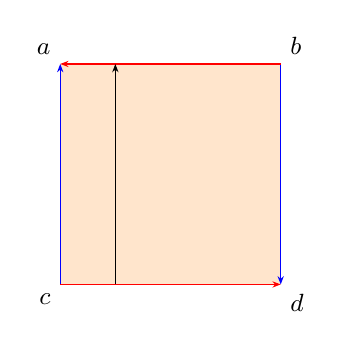
\begin{tikzpicture}[scale=1.4, >={Stealth[length=3pt]}, every node/.style={font=\small}]
  \fill[orange!20] (0,0) rectangle (2,2);
  \draw[blue, ->] (0,0) -- (0,2);
  \draw[blue, ->] (2,2) -- (2,0);
  \draw[red, ->] (0,0) -- (2,0);
  \draw[red, ->] (2,2) -- (0,2);
  \node[above left] at (0,2) {$a$};
  \node[above right] at (2,2) {$b$};
  \node[below left] at (0,0) {$c$};
  \node[below right] at (2,0) {$d$};
  \draw[->] (0.5,0) -- (0.5,2);
\end{tikzpicture}
\end{document}
